\subsection{Cyclic \suldiox~Hydrate Structures}

Having examined the bonding coordinations and bonding behavior of \suldiox~with surface waters, we now turn to a secondary behavior of the hydrate structures that form around the surface-bound \suldiox~molecule. The simulation trajectory data was analyzed to determine the presence and characteristics of \suldiox~cyclic hydrate structures that form during MD, as posited earlier and depicted in Figure \ref{fig:cyclic-structures}. Only the most commonly occuring subset of the cyclic structures were analyzed. 

\begin{figure}[h!]
	\begin{center}
		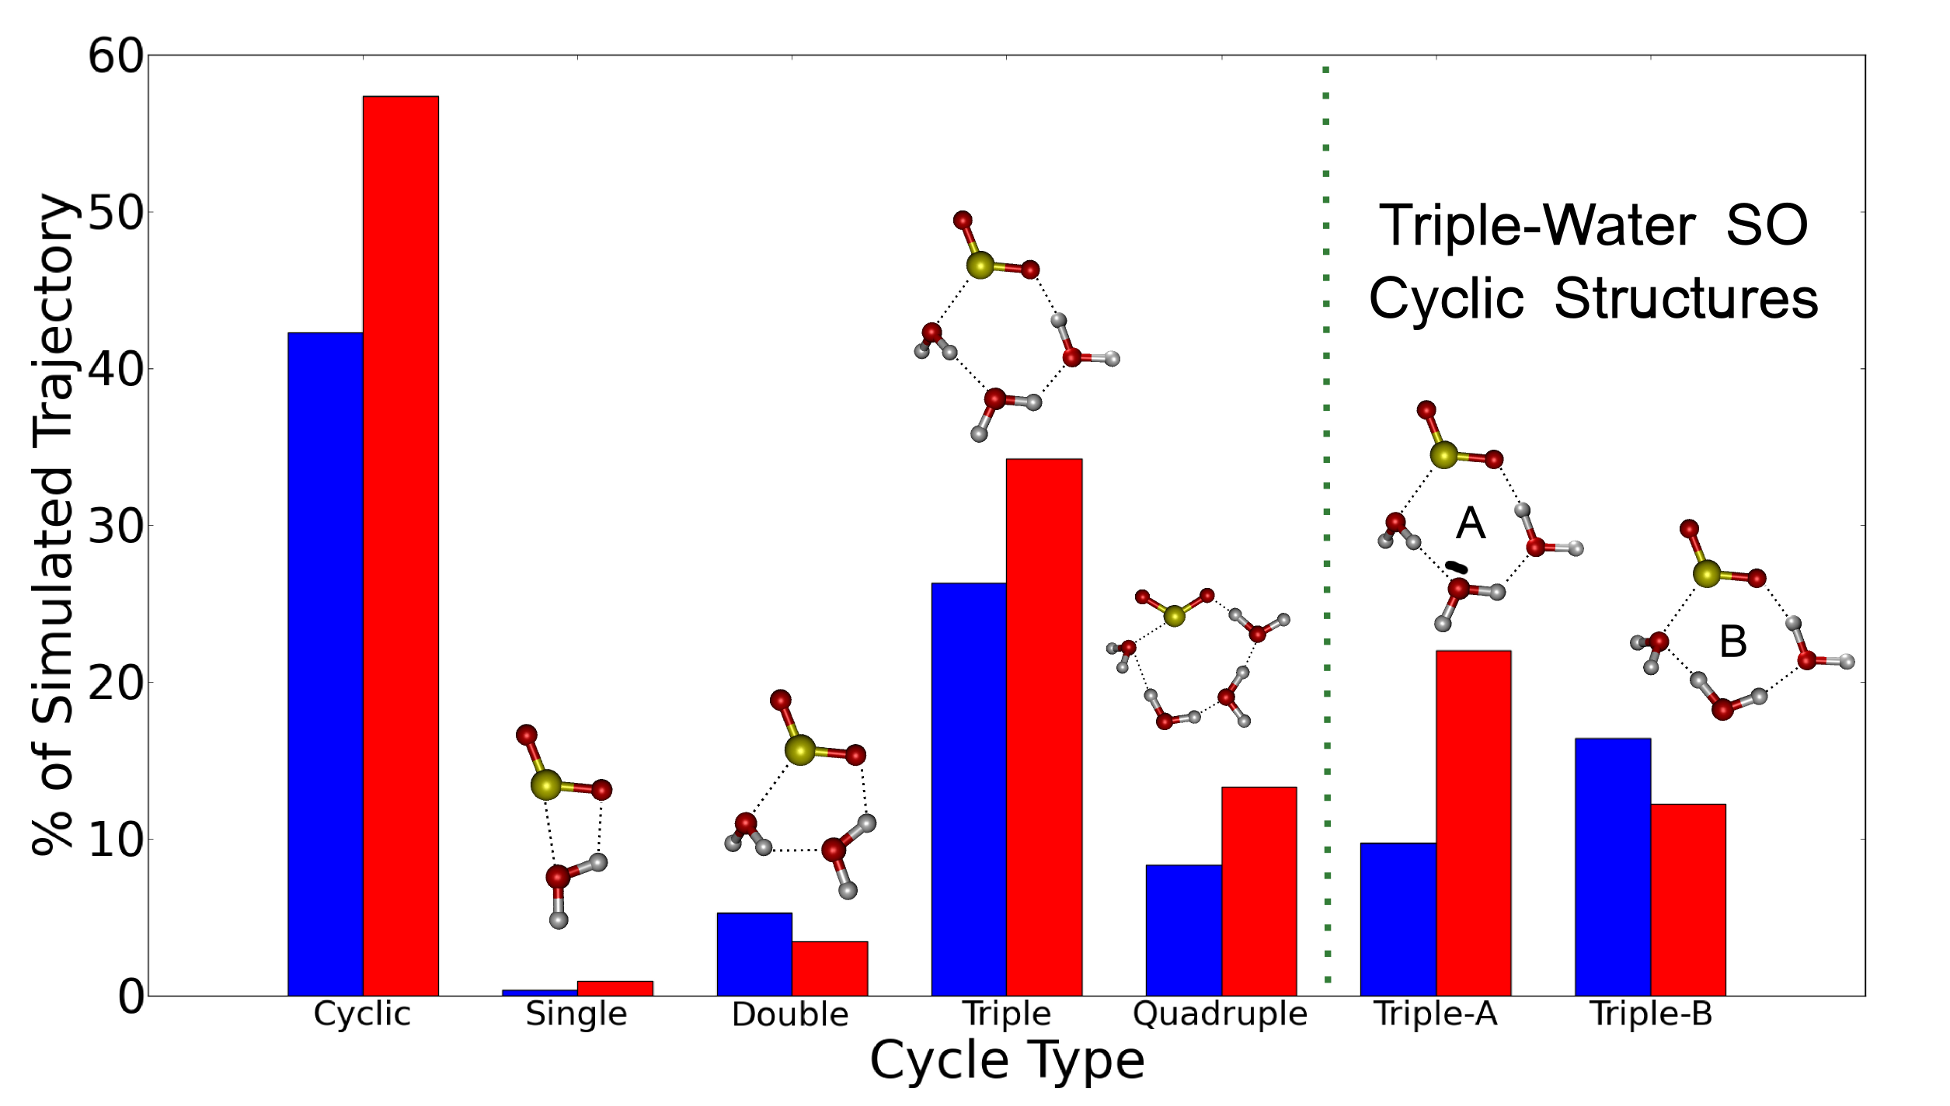
\includegraphics[scale=1.0]{images/cycles/SO-cycle-breakdown-with-cartoons-small.png}
		\caption{}
		\label{fig:cyclic-breakdown}
	\end{center}
\end{figure}
The plot in Figure \ref{fig:cycle-breakdown} shows the distribution of how often the various types of cyclic hydrates were encountered at both cold (blue) and hot (red) temperatures. Each data point shows a percentage of the MD trajectories in which the \suldiox~was a member of a cyclic structure, for different numbers of cyclic waters (up to 4). The two tallest data points, left-most in the plot, show the overall time spent in all types of cyclic structures. Clearly the hot system \suldiox~spends more time in a cyclic structure than at the cold temperature. The plot is based on two criteria for determining if a cyclic structure has formed. (1) The distances between atoms must match the same bonding/distance criteria as used for determining bonding coordinations. (2) The \suldiox~must be minimally in a bonding coordination of type ``SO'', meaning that the sulfur has at least one bonding interaction, and at least one hydrogen-bond must have formed with an oxygen to a neighboring water-hydrogen. As noted earlier in the discussion of the graph-finding routine and the BFS algorithm, the cyclic structures found represent the smallest cycles in which the \suldiox~is a member, based on order of discovery. The \suldiox~will be inevitably involved in other larger and more extended cyclic bonding structures beyond the first one discovered via the BFS. The larger and more extended cyclic structures involving more waters affect the behavior of the hydrogen-bonding network of the water surface. However, we focus here only on the smallest cycles involving the \suldiox~as the most affect the \suldiox~bonding and hydrating behaviors.

It is remarkable that the difference of the time spent in a cyclic structure between the two temperatures is 15\% (42\% cold, 57\%hot). The hot \suldiox~spends well over half of the simulated time bound as one of the hydrate cycles, and the cold \suldiox~spends just under half of the time as such. Thus, in addition to having found the most likely bonding coordination during the simulated life of \suldiox, we have also found that the hydrates of the \suldiox~form a cyclic structure for much of the time it is bound to the water surface.

Now we look at the different types of cyclic hydrates, distinguished by the number of waters involved in the bonding structure. In Figure \ref{fig:cyclic-breakdown} the single and double water cycles are the least frequently encountered structures, accounting for less than 10\% of both temperature simulations. Formation of the single type is likely energetically unfavorable because of the proximity of the single water to the \suldiox. The double-water structure was one of two types of clusters proposed in a previous computational work as a candidate structure contributing to the overall IR spectrum of surface-bound \suldiox.\cite{Baer2010} In the static and geometry-optimized cluster calculations, lacking the extended water structure or bonding from waters external to the hydrate, both the double and triple types appear equally likely to form. However, the MD simulations here have introduced many waters into a dynamic environment allowing for extended bonding networks, and the results show clearly that the double-water cyclic hydrate is formed much less often (less than 5\% at both temperatures) than the triple-water form.

The results for triple and quadruple-water structures show that larger hydrate cycles are favored at higher temperatures. Although the higher number of hydrating waters (>4) are not shown, those contribute minimally to the overall distribution. The majority of the cyclic hydrates are formed with three waters in the triple type. This hydrate type matches the bonding structure inferred from our previous experiments, and also one of the cluster types modeled by others.\cite{Tarbuck2005,Tarbuck2006,Baer2010} It was further found that of the triple-type hydrate cycles, the waters contributing to the cycles can be arranged in two ways that preserve the hydrogen-bonding between the molecules. The two triple cycle structure are depicted on the right side of Figure \ref{fig:cyclic-breakdown}, along with the plots of the contributions to the overall distribution. It is notable that each temperature has a different dominant type of triple-water cyclic structure. The cold system forms more of the type-B, and the hotter system forms primarily triple type-A.

\subsection {Cyclic Structure Energy Calculations}

\subsection {Cyclic Hydrate Structure Lifetimes}

Knowing that the \suldiox~bound to a water surface is most likely in the ``SO'' bonding coordination, and also often taking part in some type of cyclic structure, how long does the cyclic hydrate form before breaking to an acyclic structure? To answer the questions of cyclic lifespans, a method was devised to define a lifetime of a cycle. For each trajectory, the coordinate data was analyzed to determine if a cyclic hydrate structure was formed based on the bonding distance criteria established earlier in this manuscript. A timeline was then produced where each timestep was given a value of 1 or 0 if a \suldiox~cycle was found or not found, respectively. This resulted in a time-function, $C(t)$, similar in nature to a digital signal, as shown in black in Figure \ref{fig:debouncing}. Because 
